\documentclass[Space_Shuttle_Ultra_Manual.tex]{subfiles} 
\begin{document}

\section{SSU SYSTEMS}
\begin{multicols*}{2}
\renewcommand{\cfttoctitlefont}{\bf}
\localtableofcontents
\noindent
\\
%This section discusses in greater detail each of the orbiter systems that are currently simulated. The subsections are organized alphabetically, with detailed internal table of contents provided for each.\\
This section discusses in greater detail each of the space shuttle systems that are currently simulated.\\
\\
These are not meant to provide all information about the real orbiter system but to provide a working knowledge required to understand what is happening in the simulation. For full, detailed reading, each subsection provides references to relevant sections in the Shuttle Crew Operations Manual (SCOM) and should be read for a better understanding for that system.
\end{multicols*}

\subsection{External Tank (ET)}
\begin{figure}[b!]
  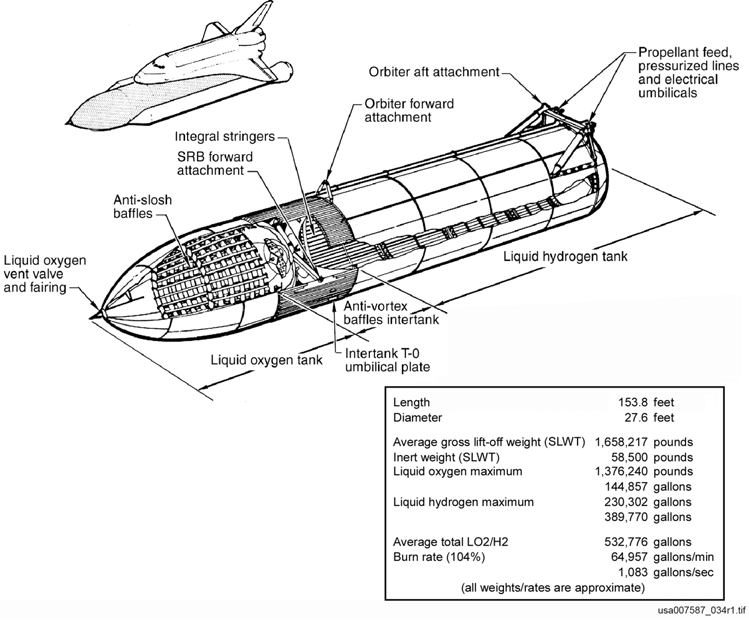
\includegraphics[width=1.0\textwidth]{SLWT.png}
  \caption{External Tank}
  \label{fig:ET}
\end{figure}
\begin{multicols*}{2}
\renewcommand{\cfttoctitlefont}{\bf}
\localtableofcontents
\subsubsection{Description}
The External Tank (ET) holds the liquid hydrogen and liquid oxygen propellants for the Main Propulsion System, and serves as a backbone for the whole space shuttle vehicle.\\
There are 3 versions of ETs$\colon$\\
$\Rightarrow$ Standard Weight Tank (SWT), the original ET to which can be added a cover of Fire Retardant Latex (FRL) paint;\\
$\Rightarrow$ Light Weight Tank (LWT), lighter weight ET resulting from structural changes;\\
$\Rightarrow$ Super Light Weight Tank (SLWT), further weight reductions to improve payload capability.\\
The scenario file entries needed to define the ET vessel are covered in Section \ref{sec:scenario-files} of this manual.
\end{multicols*}

\subsection{Solid Rocket Boosters (SRB)}
\begin{figure}[b!]
  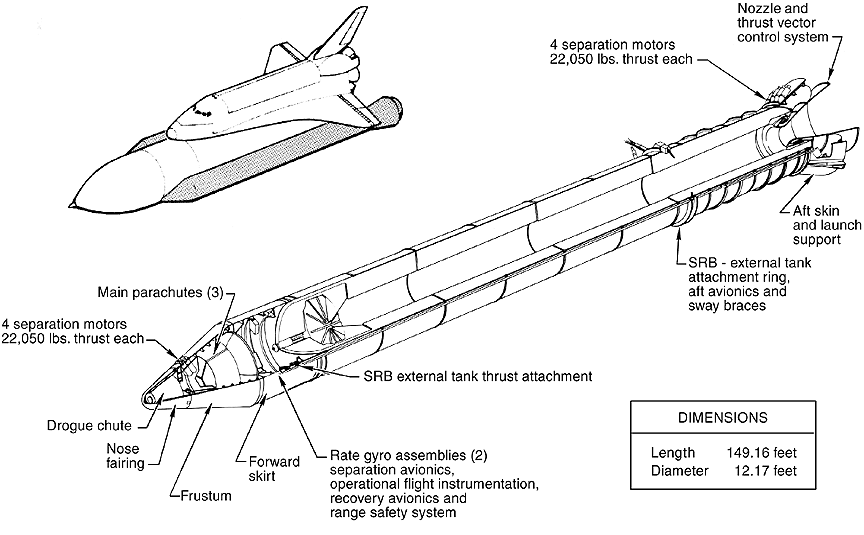
\includegraphics[width=1.0\textwidth]{SRB.png}
  \caption{Solid Rocket Booster}
  \label{fig:SRB}
\end{figure}
\begin{multicols*}{2}
\renewcommand{\cfttoctitlefont}{\bf}
\localtableofcontents
\subsubsection{Description}
The Solid Rocket Boosters (SRB) are solid propellant rockets that provide thrust during the early phases of the launch. The main component of the SRB is the Solid Rocket Motor (SRM).\\
There are 4 types of SRMs$\colon$\\
$\Rightarrow$ Standard Performance Motor (SPM), the original SRM (not yet available in SSU);\\
$\Rightarrow$ High Performance Motor (HPM), upgrade to the SPM;\\
$\Rightarrow$ Filament Wound Case (FWC), lighter case SRM planned to be used from SLC-6;\\
$\Rightarrow$ Redesigned Solid Rocket Motor (RSRM), developed in response to the Challenger accident.\\
The scenario file entries needed to define the SRB vessels are covered in Section \ref{sec:scenario-files} of this manual.
\end{multicols*}

\subsection{Auxiliary Power Unit/Hydraulics (APU/HYD)}
\begin{multicols*}{2}
\renewcommand{\cfttoctitlefont}{\bf}
\localtableofcontents
\subsubsection{Description}
The orbiter has three independent hydraulic systems. Each system provides hydraulic pressure during launch and entry to control the SSMEs, the Orbiter's aerosurfaces, and other systems.
The APUs are started 5 minutes before launch and shut down shortly after MECO.
The day before entry, a single APU is started for the FCS checkout.
A single APU is started 5 minutes before the deorbit burn (this is done to ensure at least 1 APU is functioning before committing to entry). The remaining APUs are started 13 minutes before Entry Interface.
All 3 APUs are shut down after landing.
\end{multicols*}

\subsection{Main Propulsion System (MPS)}
\begin{multicols*}{2}
\renewcommand{\cfttoctitlefont}{\bf}
\localtableofcontents
\subsubsection{Description}
The Main Propulsion System (MPS) is composed of the External Tank that holds the propellants, 3 Space Shuttle Main Engines (SSME) that provide thrust during the whole launch, and propellant manifolds to carry the propellants from the tanks to the engines.
\subsubsection{Space Shuttle Main Engines (SSME)}
The SSMEs are high performance liquid propellant rocket engines located in the aft compartment of the orbiter. They can operate between 67\% and 109\% of their rated thrust (370000lbs), and are throttled down temporarily early in the ascent to reduce aerodynamic loads on the vehicle, and then again late in the ascent to keep the acceleration under 3g.
\subsubsection{MPS Dump}
Following MECO and ET separation, the MPS Dump is automatically started to vent remaining MPS propellants from the engines and the manifolds. Liquid oxygen is vented thru the SSMEs and the liquid hydrogen is vented thru the backup LH2 dump valves and thru the fill and drain valves located on the port sidewall of the orbiter.
\end{multicols*}

\subsection{Data Processing System (DPS)}
\begin{multicols*}{2}
\renewcommand{\cfttoctitlefont}{\bf}
\localtableofcontents
\noindent
\\
The DPS consists of the shuttle's General Purpose Computers (GPCs), associated systems, and the software run by the GPCs. The 11 MDUs (Multifunction Display Units) are also part of the DPS.
\subsubsection{GPCs}
The real shuttle has 5 identical computers. Up to 4 of the 5 GPCs run the Primary Avionics Software System (PASS). The remaining computer runs the Backup Flight System (BFS). The PASS software is further divided into 3 Major Functions: \textit{GNC} (Guidance, Navigation \& Control), \textit{SM} (Systems Management) and \textit{PL} (Payload) software. The \textit{GNC} software is responsible for controlling the orbiter during flight. During critical phases of flight, such as launch and entry, multiple GPCs will run the PASS \textit{GNC} software simultaneously; this provides redundancy if one of the GPCs fails. The \textit{SM} software monitors various orbiter systems. The \textit{PL} software is not used during flight. The BFS was written separately from the PASS, and implements a subset of the PASS \textit{GNC} functions. The BFS is meant to be used in the event of a PASS failure. \\
\\
The \textit{GNC} major function is divided into multiple OPS. Each OPS represents a different phase of flight. OPS 1 is used for launch, OPS 2 is used on-orbit, and OPS 3 is used for deorbit and entry. The GPC only has enough memory to store one OPS at a time, so the PASS software is divided into multiple memory configurations. Each memory configuration contains one OPS (except for MC 1, which is used during launch, and contains both OPS 1 (launch) and OPS 6 (RTLS)). To change from one OPS to another, the appropriate memory configuration has to be loaded onto the GPCs.
Each OPS is further divided into Major Modes, which relate to specific phases of the mission. For example, OPS 2 (on-orbit) has 2 Major Modes: MM 201 (orbit coast) and MM 202 (Mnvr Exec). MM 202 is used for performing OMS burn, while MM 201 is used otherwise.
\\
At the moment, SSU only simulates the PASS \textit{GNC} software. Also, loading different memory configurations into the GPCs is not simulated. SSU assumes only one GPC is running, and does not simulate multiple GPCs performing the same operations as part of a redundant set.
\subsubsection{Multifunction Display Units (MDUs)}
The shuttle originally had 4 CRT displays, and multiple analog instruments.
The CRTs allowed the crew to interact with the shuttle computers, while the analog instruments displayed subsystem status and flight instruments.
Starting with STS-101, the analog instruments were replaced with the MDUs.
The shuttle has 11 MDUs: CDR 1 and 2 on panel F6; CRT 1, 2, and 3, and MFD 1 and 2 on panel F7; PLT 1 and 2 on panel F8; CRT 4 on panel R11; and AFD 1 in the aft station.
In real life, the MDUs display either DPS displays, flight instrument displays, or subsystem status displays.
The flight instruments and subsystem status displays replace the analog instruments, while the DPS displays are almost identical to the CRT displays.\\
\\
In SSU, each MDU is an Orbitersim MFD. CRT MFD, which is part of SSU, simulates the shuttle MEDS displays. In the future, SSU will only display accurate displays in the MDU; some displays have not been implemented yet, and so Orbitersim MFD equivalents have to be used.
Section \ref{sec:dps-displays} describes the DPS displays that have been implemented so far.
The 3 subsystem status displays (\textit{OMS/MPS}, \textit{APU/HYD} and \textit{SPI}) have been implemented in CRT MFD.
The flight instrument displays are only partially implemented. All displays in the Ascent/Entry Primary Flight Display are working except for the ADI and HSI.
\end{multicols*}

\subsection{DPS Displays}
\begin{multicols*}{2}
\renewcommand{\cfttoctitlefont}{\bf}
\localtableofcontents
\label{sec:dps-displays}
\noindent
\\
The NASA DPS Dictionary describes each display in detail. This section lists the displays that have been implemented so far and describes the differences between the real shuttle and the SSU implementation.

\begin{table*}[tb]
  \centering
  \begin{tabular}{l | c l l}
    \textbf{SITE} & \textbf{Location} & \textbf{PRI RWY} & \textbf{SEC RWY} \\
    \hline
    1 & KSC & KSC 15 & KSC 33 \\
    3 & Moron & MRN 20 & MRN 02 \\
    13 & Moron & MRN 20 & MRN 02 \\
    20 & St. John's International & YYT 29 & YYT 11 \\
		21 & Gander & YQX 21 & YQX 31 \\
		22 & Banjul & BYD 32 & BYD 14 \\
    23 & Lajes & LAJ 15 & LAJ 33 \\
    24 & Vandenberg AFB & VBG 30 & VBG 12 \\
		26 & Shannon & INN 06 & INN 24 \\
    29 & Istres & FMI 33 & FMI 15 \\
    32 & Diego Garcia & JDG 31 & JDG 13 \\
    33 & RAAF Amberley/Tindall & AMB 15 & PTN 14 \\
    36 & Bermuda & BDA 30 & BDA 12 \\
    38 & Easter Island & EIP 28 & EIP 10 \\
    39 & Hao Atoll & HAO 12 & HAO 30 \\
    45 & Edwards AFB & EDW 22 & EDW 04
  \end{tabular}
  \caption{Landing Site Table}
  \label{tab:LandingSites}
\end{table*}

\subsubsection{ASCENT TRAJ}
\begin{figure}[H]
  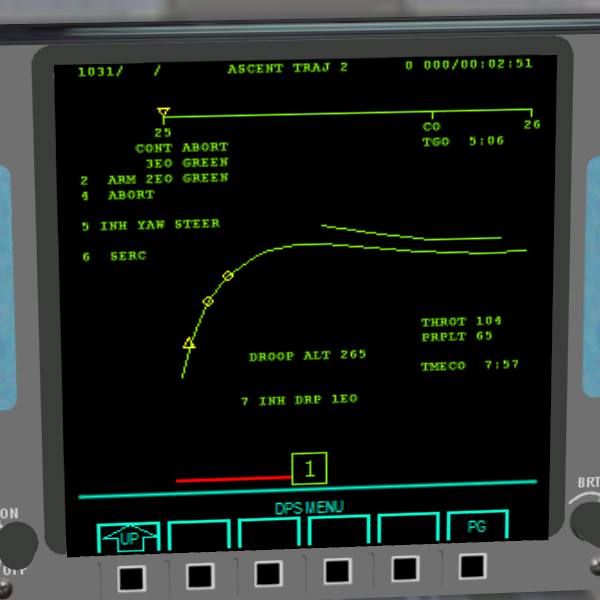
\includegraphics[scale=0.5]{ASCENTTRAJ2.png}
  \caption{ASCENT TRAJ display}
  \label{fig:ASCENT_TRAJ}
\end{figure}
This display is used in MM 102 and MM 103 to monitor the vehicle's trajectory during ascent. The DROOP ALT digital output is not being driven. The ITEMs on this display are related to abort options and are not supported by SSU.

\subsubsection{UNIV PTG}
This display is used in MM 201, and is used to control the attitude of the orbiter. Most of the functions in this display have been implemented. ITEM 8 (TGT ID) only supports an entry of 2 at the moment, and ITEMS 9-13 are not supported. ITEM 20 (TRK) is not supported. Finally, ITEMs 22-24 (which affect how the attitude error is displayed) are not implemented.

\subsubsection{OMS MNVR EXEC}
This display is used in MM 104 (OMS 1 MNVR EXEC), MM 105 (OMS 2 MNVR EXEC), MM 106 (OMS 2 MNVR COAST), MM 202 (ORBIT MNVR EXEC), MM 301 (DEORB MNVR COAST), MM 302 (DEORB MNVR EXEC) and MM303 (DEORB MNVR COAST). It is used mainly to perform OMS engine burns to change the shuttle's orbit.
This display is almost completely implemented in SSU. ITEMs 28-40 (OMS gimbal check, FWD RCS dump and SURF DRIVE) have not been implemented yet.

\subsubsection{DAP CONFIG}
This display is used in MM 201 and MM 202, and control the Digital Autopilot (DAP) settings. In real life, there are 15 DAP A configurations and 15 DAP B configurations; at any time, 1 DAP A and 1 DAP B configuration is active, and the crew selects between DAP A and B using the PBIs on Panels C3 and A6. In SSU, there is only 1 DAP A configuration and 1 DAP B configuration. As a result, ITEMS 1 and 2 (which select the active DAP A \& B configuration) are not implemented. Also ITEMs 3 and 4 (which, in real life, select a DAP configuration and load it into the EDIT column) simply select between loading DAP A and DAP B into the EDIT column.

\subsubsection{ORBIT TGT}
This display is used in MM 201 and MM 202 to compute rendezvous burns. In real life, the state vectors for the rendezvous target are uploaded from Mission Control. In SSU, the name of the target vessel is specified in the scenario file.
% TODO: reference scenario file
The real-life ORBIT TGT display can load rendezvous targets by specifying a TGT NO (ITEM 1); in SSU, each parameter has to be set individually. SSU doesn't support the EL parameter (ITEM 6), which allows the burn TIG to be computed to match a desired elevation angle; instead, the TIG must be specified.
SSU can only be used to compute the T1 burn (ITEM 28), and not the T2 burn. In real life, the T2 burn computations are not used.

\subsubsection{ENTRY TRAJ}
\begin{figure}[H]
  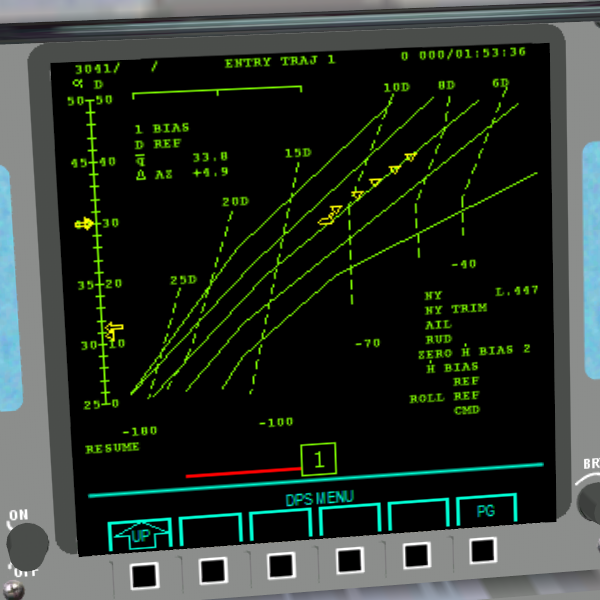
\includegraphics[scale=0.5]{ENTRYTRAJ1.png}
  \caption{ENTRY TRAJ display}
  \label{fig:ENTRY_TRAJ}
\end{figure}
These displays are used during entry to monitor the vehicle's trajectory. Currently the only digital outputs being driven are the q-bar, delta-AZ and NY outputs. The guidance box and trailers are not displayed, the phugoid scale is not driven and no item entries are supported.

\subsubsection{VERT SIT}
\begin{figure}[H]
  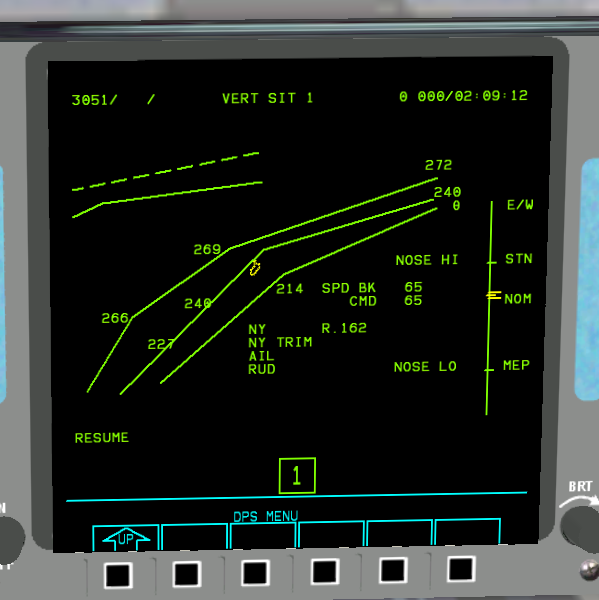
\includegraphics[scale=0.5]{VERTSIT1.png}
  \caption{VERT SIT display}
  \label{fig:VERT_SIT}
\end{figure}
These displays are used during TAEM to monitor the vehicle's trajectory. Currently the only digital outputs being driven are the SPD BK, SPD BK CMD and NY outputs. The Theta scale and the E/W scale are not driven.

\subsubsection{HORIZ SIT}
\begin{figure}[H]
  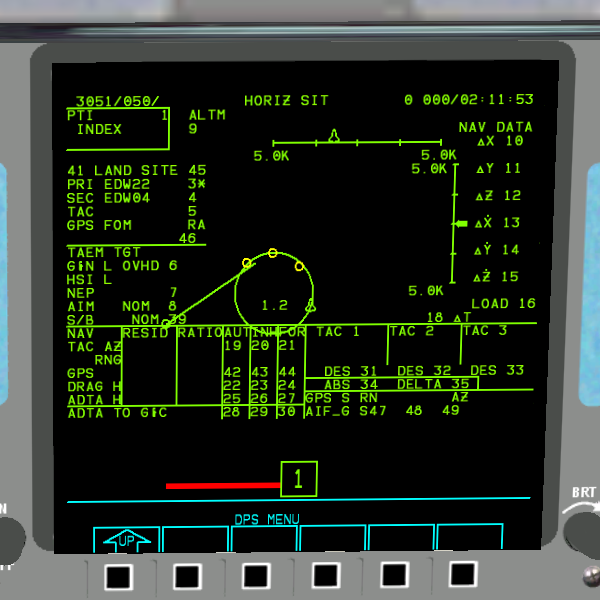
\includegraphics[scale=0.5]{HORIZSIT.png}
  \caption{HORIZ SIT display}
  \label{fig:HORIZ_SIT}
\end{figure}
This display is used during deorbit and entry to specify the landing site and monitor the position of the shuttle relative to the HAC and the runway.
The HORIZ SIT display in SSU is simplified compared to the real life version.
Currently the vertical error scale is not driven prior to A/L interface, and only ITEMs 3, 4, 6, 8, 39 and 41 are supported. 
ITEM 41 selects the landing site, ITEMs 3 and 4 switch between the primary and secondary runway. ITEM 6 switches between a straight-in and overhead approach, ITEM 8 switches the aim point between nominal and close, and ITEM 39 switches between nominal, short and ELS (Emergency Landing Site) speedbrake configurations for final approach.
These parameters all affect the entry autopilot, so they should be set before Entry Interface (EI).
Table \ref{tab:LandingSites} shows the list of landing sites currently supported by SSU.
\end{multicols*}

\subsection{MEDS Displays}
\begin{multicols*}{2}
\renewcommand{\cfttoctitlefont}{\bf}
\localtableofcontents
\label{sec:meds-displays}

\subsubsection{A/E PFD}
\begin{figure}[H]
  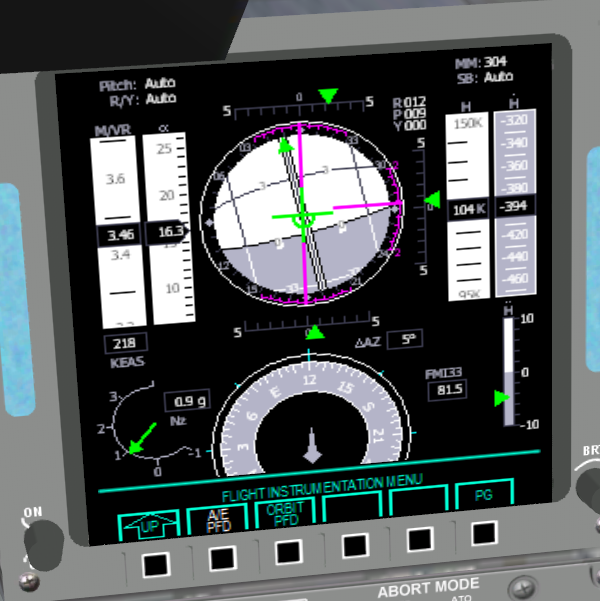
\includegraphics[scale=0.5]{AEPFD.png}
  \caption{A/E PFD}
  \label{fig:AE_PFD}
\end{figure}
The A/E PFD display shows several parameters relevant to Ascent and Entry. Currently the attitude error needles are not properly driven, so they are not to be trusted. The ADI is operating in LVLH mode only with yaw zeroed, so the ADI ATT switches have no effect. During TAEM, and up until A/L interface, the vertical position error is not being driven, and the heading error is not being driven. The HSI is missing all the bearing pointers, and during launch it is not referenced from the target plane. The X-Trk value is not being driven.
OMS/MPS
The OMS/MPS display provides information about various pressures in the OMS and MPS systems. The OMS He TK P and N2 TK P meters are not driven.

\subsubsection{ORBIT PFD}
\begin{figure}[H]
  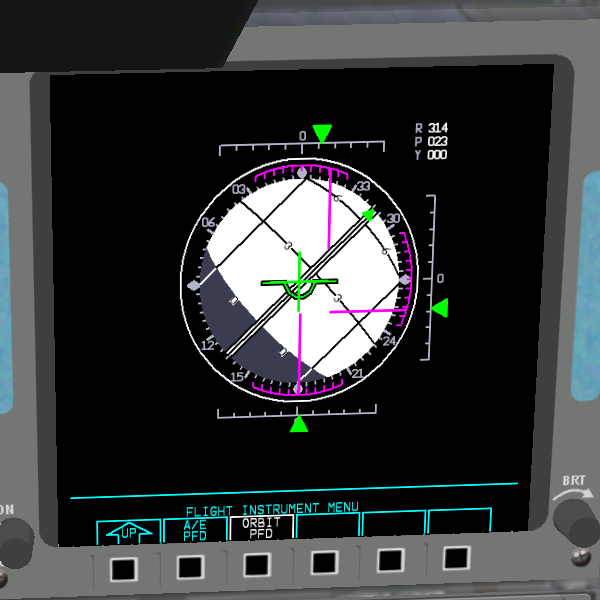
\includegraphics[scale=0.5]{ORBITPFD.png}
  \caption{Orbit PFD}
  \label{fig:Orbit_PFD}
\end{figure}
The Orbit PFD is used for on-orbit display of vehicle attitude. Currently the attitude error needles currently are not being driven properly, so they are not to be trusted. The ADI currently operates only in the LVLH mode with yaw zeroed, so the ADI ATT switches have no effect.
\end{multicols*}

\begin{multicols*}{2}
\subsubsection{OMS/MPS}
\begin{figure}[H]
  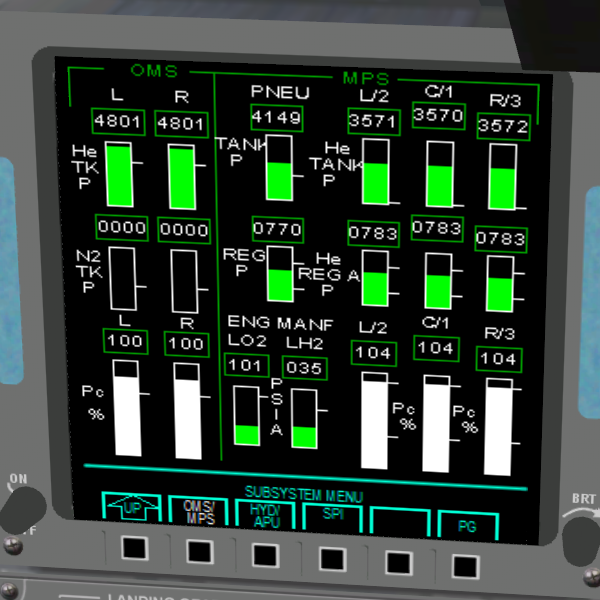
\includegraphics[scale=0.5]{OMSMPS.png}
  \caption{OMS/MPS display}
  \label{fig:OMS_MPS_MEDS}
\end{figure}
The OMS/MPS display provides information about various pressures in the OMS and MPS systems. The OMS He TK P and N2 TK P meters are not driven.

\subsubsection{APU/HYD}
\begin{figure}[H]
  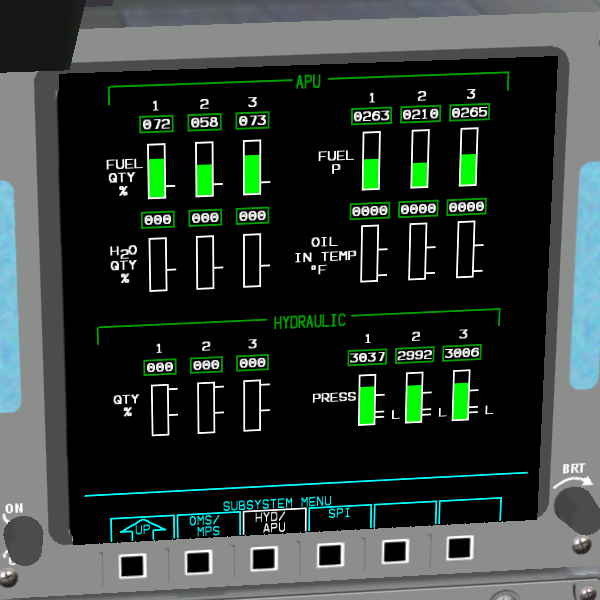
\includegraphics[scale=0.5]{HYDAPU.png}
  \caption{APU/HYD display}
  \label{fig:APU_HYD_MEDS}
\end{figure}
The APU/HYD display shows pressures, quantities and temperatures related to the hydraulic system. The APU H2O QTY \%, OIL IN TEMP $^\circ$F and HYDRAULIC QTY \% meters are not driven.

\subsubsection{SPI}
\begin{figure}[H]
  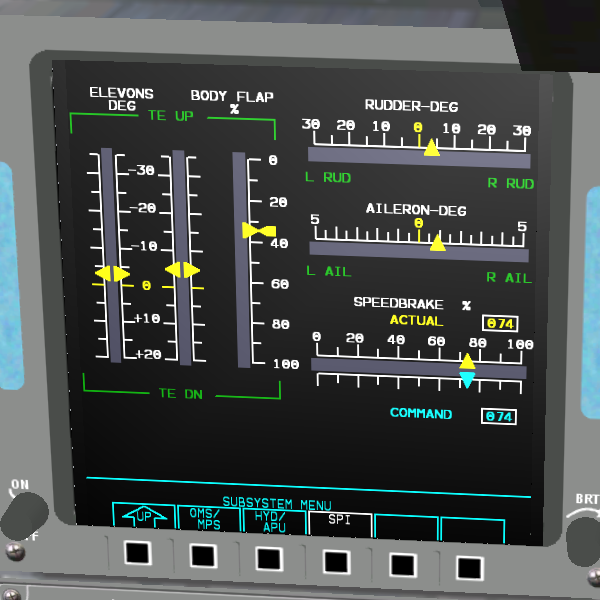
\includegraphics[scale=0.5]{SPI.png}
  \caption{SPI display}
  \label{fig:SPI_MEDS}
\end{figure}
The SPI display shows the position of the orbiter's aerosurfaces. The BODY FLAP \% indicator is non-functional.
\end{multicols*}

\begin{multicols*}{2}
\subsection{Launch Pads}
SSU can be launched from 2 launch pads: Launch Complex 39 (LC39) at the Kennedy Space Center in Florida, or Space Launch Complex 6 (SLC-6) at the Vandenberg Air Force Base in California.
\begin{figure}[H]
  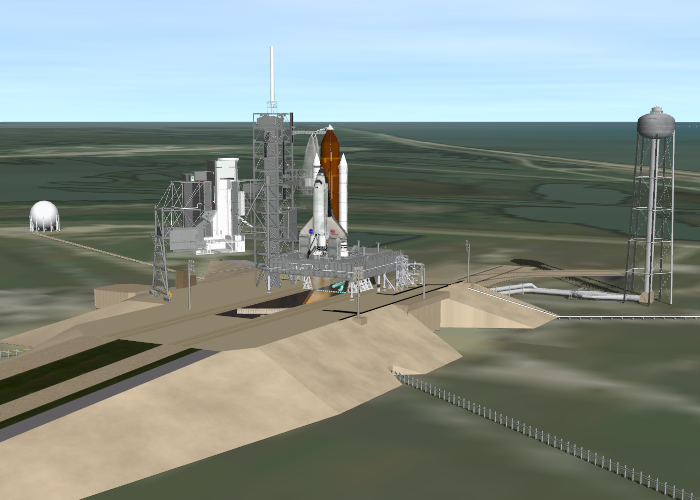
\includegraphics[width=0.5\textwidth]{LC39.png}
  \caption{Launch Complex 39}
  \label{fig:LC39}
\end{figure}
\begin{figure}[H]
  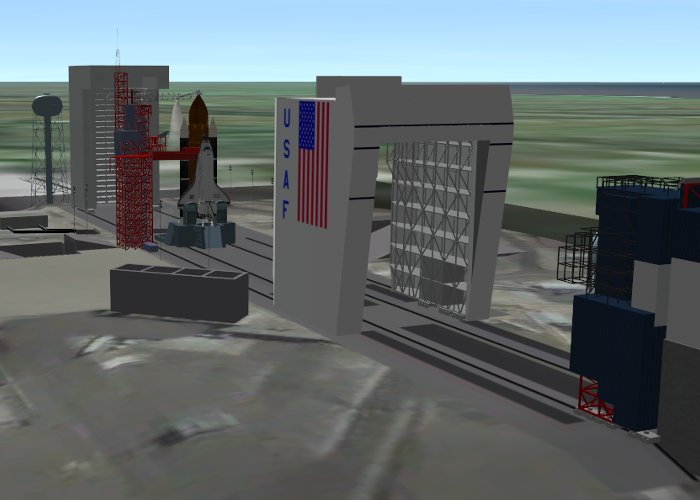
\includegraphics[width=0.5\textwidth]{SLC6.png}
  \caption{Space Launch Complex 6}
  \label{fig:SLC6}
\end{figure}
\noindent
Most pad structures are controlled automatically during the countdown, but manual control is available for all of them via a dialog window which is opened by the keys Ctrl+Space.\\
%Most pad structures are controlled automatically during the countdown, but all can be controlled manually via a dialog window which is opened by the keys Ctrl+Space.\\
The scenario file entries needed to define the launch pad vessels are covered in Section \ref{sec:scenario-files} of this manual.
\end{multicols*}

\end{document}
